% REV00 Tue 20 Jul 2021 08:12:01 WIB
% START Tue 20 Jul 2021 08:12:01 WIB

\chapter{Keenam}

% 11
\begin{figure}[htbp]
% h: here, where the figure appears in the text (use can always just use [h] )
% t: top,  top of the current page.
% b: bottom of the current page.
% p: page, top of the next available float space (sometimes end up being the end of the document).
\centerline{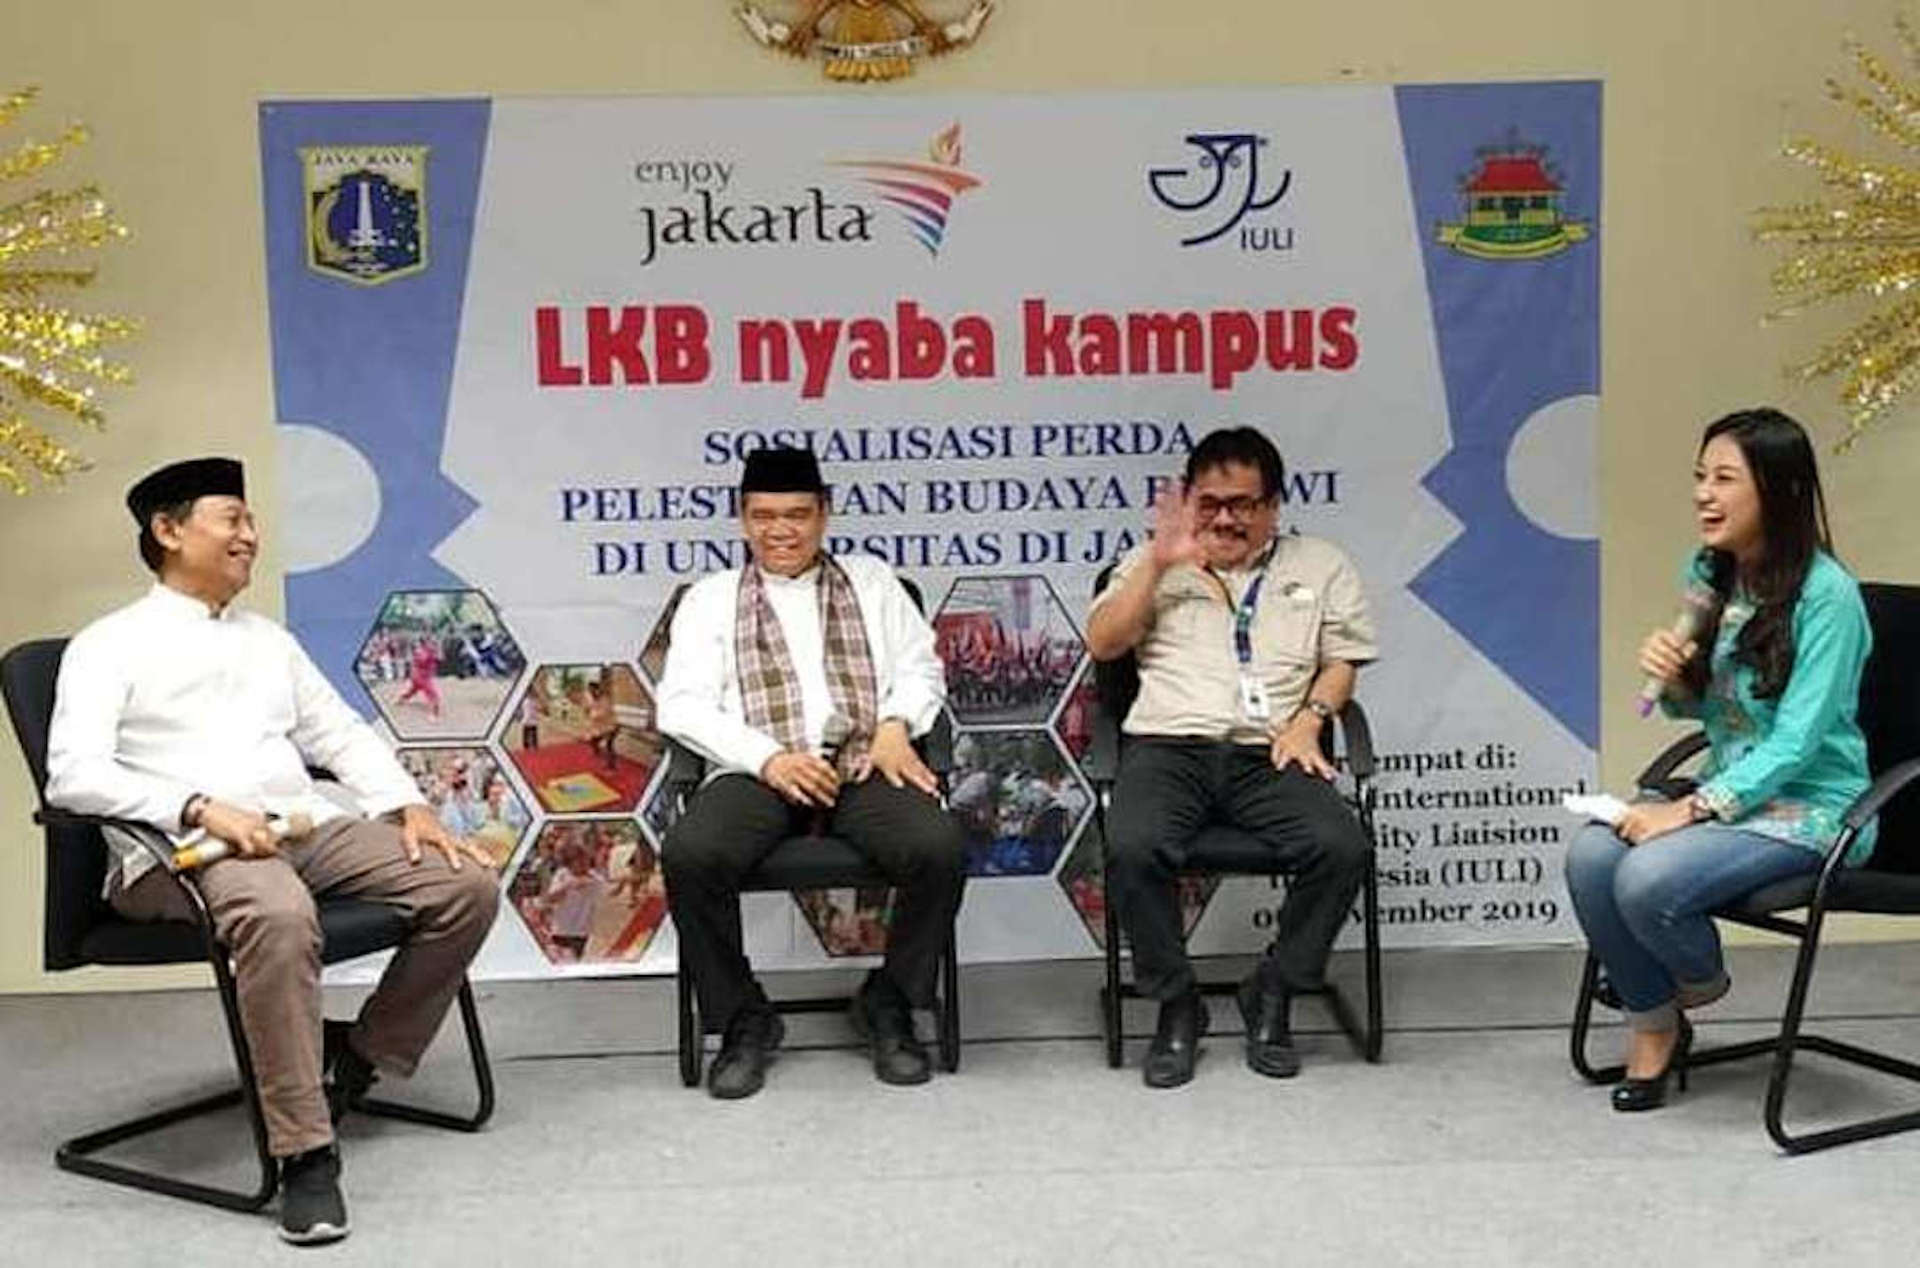
\includegraphics[scale=1.0]{01-06-01}}
\caption{“Satiri mendekatkan Kampus IULI, DKI dan budaya Betawi”. Sumber: FB Satiri M Zen.}
\label{01-06-01}
\end{figure}
%

Malam itu ia tiba di rumah sekitar jam sembilan. Ah, masih ada waktu buat si doi pujaan hati. Dibawalah gitar Pos Ronda langsung menuju rumah sang pacar, Fitria. Jrengg…

\begin{verbatim}
"... Sungguh karena dia
Aku di depan anda
Memberanikan diri
Bergaya dan bernyanyi

Pandangan pertama
Awal aku berjumpa
Pandangan pertama
Awal aku berjumpa…”
\end{verbatim}

Ya ampuun, itu lagu dangdut, eh, nasional, paling top saat itu, “Pandangan Pertama” oleh A. Rafiq. Satiri tahu, sang pujaan belum tidur, karena lampu kamarnya terlihat masih dihidupkan. Kode penantian sang pacar. Manalah dia berani masuk ke rumah gedongan itu. Babanya Fitria galak. Selagu belum selesai, tiba-tiba…

“Hoi, lu ngapain ngamen depan rumah orang malem-malem begini!,” Satiri langsung ngacir… (“Gosh what are you doing man!” and then Satiri run away at once. Gosh…)

Ya sudah, yang penting sudah kirim lagu buat sang pujaan hati. Pasti dia senyum-senyum sendiri kegirangan di kamarnya. Walaupun babanya tadi sempat ngamuk.

Kembali ke rumahnya, Satiri merenungkan kembali kata-kata Jendral O. Mengapa dia tidak menjawabnya secara langsung? Sepertinya kecil harapan. Tetapi dia ingat bahwa dia tadi sudah bilang terima kasih dan cium tangan. Bersyukur.

Kemampuan untuk bersyukur dan berterima kasih adalah nikmat yang orang-orang sering menganggapnya kurang penting atau relevan. They take it for granted. Padahal sebaliknya, anda harus mengasahnya, merawatnya baik-baik.

***

Seumur hidupnya hingga SMA Satiri belum pernah meninggalkan tanah Betawi. Semua saudara ayah-ibunya adalah orang Betawi dan tinggal di Betawi. Bertanyalah dia ke banyak orang bagaimana caranya untuk sampai di Bandung. Naik bus adalah pilihan utama, lewat Bogor dan Puncak.

Kecerdasannya memudahkan ia untuk mencari kantor cabang sang Jenderal, menerima uang dan sekaligus pekerjaan, mencari kantor ITB, dan mendaftar, serta mencari kontrakan yang murah. Uang harus dihemat.

Sebagaimana perintah sang Jendral, mulailah dia keliling kampung menjual berbagai produk termasuk jam tangan. Didapatinya bahwa hal ini beda betul dengan dagang kembang.

Setiap hari selama bulan pertama itu selepas kuliah pagi atau sebelum kuliah siang dia keliling rumah-rumah padat penduduk di sekitar ITB. Dari mulai belakang UNISBA, Pasar Balubur (sekarang Baltos), Pelesiran, belakang Kebon Binatang hingga ke Lebak Gede (sekarang Sabuga). Kadang naik juga ia ke Cisitu hingga daerah Dago Atas. Kadang merambah juga dia ke Sekeola, perkampungan di depan UNPAD, yang kebetulan kontrakannya nyempil di Tubagus Ismail Bawah, persis di pinggiran kali kecil.

“Jam tangan, dompet alus, gesper, ayo ibu-bapa, teteh, mangga dicoba..” terikanya menjajakan dengan sepatah dua patah kata bahasa Sunda. Kadang dia bernyanyi dangdut untuk menghibur calon pembelinya. Ketika dia sedang capek karena barang-barangya susah laku, dia mulai berpikir: ini perusahaan produknya seperti ini marketingnya mengapa begini ya? Ah, super ngawur…

Tak lebih dari sebulan pekerjaan ini dilakoni. Di kosannya dia mendapat surat untuk menemui sang Jenderal yang kebetulan ke kantor cabang Bandung.

“Kamu fokus kuliah saja. Sampai kamu lulus. Nilai-nilaimu harus bagus, dan laporkan ke saya...”

“Kalau ada kebutuhan tambahan silahkan buat pengajuan ke Kantor Cabang."

"Kamu enggak usah dagang lagi. Penjualan kamu juga jelek!”

Horeee…

Tuhan lagi-lagi menurunkan bantuan. Tentu ini Tuhannya siapa saja yang berani mengangkat beban.

Duit sudah di tangan. Kuliah tahun pertama kan cuma perkuatan SMA plus sedikit laa. No problemo.

“Kalau begitu, mending aku bantu-bantu baba dagang kembang. Sekalian lihat-lihat Fitria yang hatinya juga sedang berkembang”.

***

Awal masuk ITB, rambutnya dibuat Punk, dengan blue jean dan kaos oblong jadi andalan. Kaos kebanggan yang itu-itu juga, tiga potong, buatan Tokema ITB.

Gaya lenongnya memukau semua anak MIPA yang cenderung serius. Karena dapat angin kadang gayanya terbawa masuk ke ruang kelas. Ini kebanalan yang ke sekian, pas dosen menjelaskan teori pada salah satu praktikum Kimia-I. Pak dosen tua, mungkin juga sudah sedikit rada-rada lupa…

“Untuk masalah ini, saya lihat dulu bukunya ya..”

“Iya Pak lihat saja dahulu bukunya Pak biar jelas,” potong satiri dengan nada jenaka… Gerrrr sekelas praktikum tertawa gempar.

“Kamu keluaaaar!!!” teriak sang dosen mengamuk…

Dari ketawa ngakak, seperti langsung disiram air es. Dengan wajab pucat dan gontai Satiri keluar lab, kecut…

Besoknya kawan-kawan berupaya menghiburnya, tapi dia masih juga bisa bercanda.

“Kalau Kimia-I ini gua lulus, gua mau buka baju guling-guling di depan lab Kimia,” katanya. Ini kayak nazar mission impossible. Sebab praktikum kimia itu cuma 6x satu semester, dan salah satunya sudah dinilai nol. Nilai kimia itu nilai ujian plus praktikum, tapi praktikumnya juga harus lulus.

Untuk diketahui, di kelas saya, hasil ujian akhir Kimia-I itu berkisar antara -5 sampai dengan 92. Ya betul: ada yang dapat minus lima. Ini ITB jaman old-school bung…

Pada akhir semester, kejadian. Tuhan mendengar janjinya itu: Satiri lulus Kimia-I. Benarlah itu terjadi di depan mata semua orang, dia buka baju terus guling-gulingan di depan lab Kimia. Waduuuh… Kebayang kaan… Makanya jangan sembarang janji yah…

Sore ketika di kosan dia teringat Fitria, sang pujaan… Pulang…
\\[10pt]

Sumber tulisan asli \url{https://www.facebook.com/reno.alamsyah.94/posts/10226511661043875}

